\appendixpage
\begin{appendices}
	\lfoot{}
	\section{Топлинно синхотронно излъчване от релативистка плазма}
	
	Механизмът на синхотронно излъчване е добре изучен (CITE HERE), но пълното му извеждане, започвайки от първи принципи (т.е. от уравненията на Максуел), трудно се намира в литературата (частични изводи могат да бъдат намерени в CITE HERE). За пълнота на изложението в този дисертационен труд, тук ще представим пълното извеждане на функциите на излъчване от свръхрелативистки заредена плазма в термодинамично равновесие.
	
	\subsection{Електромагнитни полета на ускорени заряди}
	
	Разглеждането ни ще започнем още от уравненията на Максуел за скаларния $U\left(\vec{r},t\right)$ и векторния $\vec{A}\left(\vec{r},t\right)$ потенциал във вакуум с наложена калибровка на Лоренц:
	
	\begin{equation}
		\begin{split}
		&\Box U\left(\vec{r},t\right) = \frac{\rho(\vec{r},\,t)}{\epsilon_0},\\
	    &\Box \vec{A}\left(\vec{r},t\right) = \mu_0\vec{j}(\vec{r},\,t)
		\end{split}
	\end{equation}
	Тогава решенията в цялото пространство могат да се запишат чрез закъсняващите функциите на Грийн като:
	\begin{equation}
		\begin{split}
			&U\left(\vec{r},t\right) = \frac{1}{4\pi\epsilon_0}\int_{R^3}\int_{t^{\,\prime}} \rho(\vec{r}^{\,\prime},t)\frac{\delta\left(t^\prime - \left[t - \frac{\vert \vec{r} - \vec{r}^{\,\prime}\vert}{c}\right]\right)}{\vert \vec{r} - \vec{r}^{\,\prime}\vert}dt^\prime d^3\vec{r}^{\,\prime}\\
			&\vec{A}\left(\vec{r},t\right) = \frac{\mu_0}{4\pi}\int_{R^3}\int_{t^{\,\prime}} \vec{j}(\vec{r}^{\,\prime},t)\frac{\delta\left(t^\prime - \left[t - \frac{\vert \vec{r} - \vec{r}^{\,\prime}\vert}{c}\right]\right)}{\vert \vec{r} - \vec{r}^{\,\prime}\vert}dt^\prime		d^3\vec{r}^{\,\prime} 
		\end{split}
	\end{equation} 
	
	Източниците в уравнение (A.1) характеризират излъчващата среда, но директното пресмятане на интегралите (A.2) в термини на \emph{макроскопичните} потоци на излъчващата среда е непрактично поради две основни причини:\\
	
	1) Разглежданите тук процеси на излъчване се пораждат от ускорението на заредените частици в средата. Това означава, че ако изведем закон за излъчване, базиран на макроскопични потоци, ние неизбежно пренебрегваме \emph{микроскопичната} динамика на зарядите, която в случая е значима.\\
	
	2) Базирайки се на макроскопични потоци, ние се ограничаваме до един конкретен модел на средата и не можем да правим общи феноменологични заключения.\\
	
	С оглед на това, нека се възползваме от линейността на уравненията (29) и нека представим излъчващата среда като ансамбъл от заряди $q$, движещи се по закон, описван от $\vec{r}_0(t)$. Така ще изведем законите за излъчване на \emph{една} частица от ансамбъла, и ще използваме принципа на суперпозицията за да възстановим излъчването на цялата среда. Тогава можем да запишем източниците в уравнения (29) за \emph{една} частица като:
	
	\begin{equation}
		\begin{split}
		&\rho(\vec{r},t) = q \delta\left[\vec{r} - \vec{r}_0(t)\right]\\
		&\vec{j}(\vec{r}, t) = q \vec{v}_0(t)\delta\left[\vec{r} - \vec{r}_0(t)\right],
		\end{split}
	\end{equation}
	където $\vec{v}_0(t) = \frac{d\vec{r}_0}{dt}$ e скоростта на заряда. Замествайки тези изрази в интегралите (A.2) ни позволява директно да извършим интегрирането по пространствените координати. Тогава дефинирайки следните променливи:
	\begin{equation}
		\vec{R}(t) = \vec{r} - \vec{r}_0, \quad \vec{R}_0(t) = \frac{\vec{R}(t)}{R(t)},\quad R(t) = |\vec{R}(t)|
	\end{equation}
	получаваме следните изрази:
	\begin{equation}
		\begin{split}
		&U(\vec{r},t) = \frac{q}{4\pi\epsilon_0}\int_{t^\prime}\frac{\delta\left(t - t^\prime + \frac{R(t^\prime)}{c}\right)}{R(t^\prime)}dt^\prime\\
		&\vec{A}(\vec{r},t) = \mu_0\frac{q}{4\pi}\int_{t^\prime}\vec{v}(t^\prime)\frac{\delta\left(t - t^\prime + \frac{R(t^\prime)}{c}\right)}{R(t^\prime)}dt^\prime\\
		\end{split}
	\end{equation}
	
	Въвеждаме нова интеграционна променлива, дефинирана като $\tau = t^\prime - t + \frac{R(t^\prime)}{c}$. Тогава
	\begin{equation}
		d\tau = dt^\prime + \frac{1}{c}\frac{dR}{dt^\prime}dt^\prime\rightarrow dt^\prime = \frac{d\tau}{1 - \frac{\vec{v}(t^\prime)\cdot\vec{R}_0(t^\prime)}{c}} := \frac{d\tau}{\alpha(t^\prime)}
	\end{equation}
	
	Това свежда интегралите (33) до:
	\begin{equation}
		\begin{split}
		U(\vec{r},t) = \frac{q}{4\pi\epsilon_0}\int_\tau \frac{\delta(\tau)}{\alpha(t^\prime(\tau))R(t^\prime(\tau))}d\tau =\frac{q}{4\pi\epsilon_0} \frac{1}{\alpha(t^\prime(0))R(t^\prime(0))}\\
		\vec{A}(\vec{r},t) = q\frac{\mu_0}{4\pi}\int_\tau \frac{\vec{v}(t^\prime(\tau))\delta(\tau)}{\alpha(t^\prime(\tau))R(t^\prime(\tau))}d\tau=\mu_0\frac{q}{4\pi} \frac{\vec{v}(t^\prime(0))}{\alpha(t^\prime(0))R(t^\prime(0))}
		\end{split}
	\end{equation}
	Условието $\tau = 0$ дефинира т.н. \emph{време на закъснение} $t^\prime(\tau = 0) := t_0$, което се определя неявно от $c(t - t_0) = R(t_0)$, и представлява времето в което електромагнитно смущение трябва да бъде излъчено от източник, намиращ се тогава в точката $\vec{r}_0(t_0)$ за да се засече от наблюдател, намиращ се в точката $\vec{r}$, в момента t. В по-явен вид уравнения (A.7) могат да се запишат като:
		\begin{equation}
		\begin{split}
			U(\vec{r},t) = \frac{q}{4\pi\epsilon_0 |\vec{r} - \vec{r}_0(t_0)|} \frac{1}{1 - \frac{\vec{v}(t_0)\cdot \vec{R}_0(t_0)}{c}}\\
			\vec{A}(\vec{r},t) = \mu_0\frac{q\vec{v}(t_0)}{4\pi\epsilon_0 |\vec{r} - \vec{r}_0(t_0)|} \frac{1}{1 - \frac{\vec{v}(t_0)\cdot \vec{R}_0(t_0)}{c}},
		\end{split}
	\end{equation}
	и се наричат \emph{калибровачни потенциали на Лиенард-Вихерт}. Съответстващите електромагнитни полета се намират от:
	\begin{equation}
		\vec{E}(\vec{r},t) = -\nabla U(\vec{r},t) - \frac{\partial A}{\partial t}(\vec{r},t),\quad \vec{B}(\vec{r},t) = \nabla\times \vec{A}(\vec{r},t)
	\end{equation}
	Някой междинни резултати при пресмятането на производните в (A.9) са:
	\begin{equation}
		\begin{split}
			&\nabla t_0 = -\frac{\vec{R}_0}{\alpha c}\\
			&\nabla R = \frac{\vec{R}_0}{\alpha}\\
			&\nabla(\alpha R) = \vec{R}_0 - \frac{\vec{v}}{c} - \frac{v^2}{\alpha c^2}\vec{R}_0 + \frac{\vec{v}\cdot\vec{R}_0}{\alpha c}\vec{R}_0 + \frac{\vec{a}\cdot \vec{R}}{\alpha c^2} \vec{R}_0\\
			&\frac{\partial}{\partial t}(\alpha R) = c - \frac{c}{\alpha} + \frac{v^2}{\alpha c} - \frac{\vec{a}\cdot\vec{R}}{\alpha c},
		\end{split}
	\end{equation}
	където $\vec{a} = \frac{d \vec{v}}{dt}$ e ускорението на заряда. Тогава изразите за полетата на Лиенард-Вихерт са (дефинирайки $\vec{\beta} = \frac{\vec{v}}{c}$):
	\begin{equation}\label{LW_fields}
		\begin{split}
			&\vec{E(t)} =\left. \frac{q}{4\pi\epsilon_0}\left\{\frac{\vec{R}_0 - \vec{\beta}}{\alpha^3 R^2}\left(1 - \beta^2\right) + \frac{\vec{R}_0 \times \left[\left(\vec{R}_0 - \vec{\beta}\right)\times\dot{\vec{\beta}}\right]}{\alpha^3 c R}\right\}\right\vert_{t = t_0(t)}\\
			&\vec{B(t)} = \left. \frac{\vec{R}_0}{c}\times\vec{E}\right\vert_{t = t_0(t)},
		\end{split}
	\end{equation}
	
където дясната страна е функция на времето и е пресметната в момента $t_0$. Това е следствие от принципа за причинност. 
\newpage
\subsection{Геометрията на синхотронното излъчване}	
Полетата (А.11) притежават свойството, че имат радиационна компонента. Тя зависи силно от относителната ориентация на вектора на ускорението (на практика този на магнитното поле), вектора на скоростта и лъча на зрение, и може да се раздели на два феноменологично различни случая:\\

1) Ускорение, паралелно на скоростта - това е т.н. спирачно лъчение\\

2) Ускорение, ортогонално на скоростта - това е синхотронното излъчване, което представлява интерес за нас. В разглежданията надолу ще приемем, че лъчението е \emph{изцяло} синхотронно. Това, разбира се, е приближение, но в границата на релативиски скорости, излъчената синхотронна мощност е с множител $\gamma^2 = \frac{1}{1 - \beta^2}$ по-голяма от тази на спирачното лъчение, и следователно то може да бъде пренебрегнато.\\

Потокът на излъчената за единица време електромагнитна енергия се определя от вектора на Пойнтинг $\vec{S}$:
\begin{equation}
	\vec{S} = \frac{1}{\mu_0}\vec{E}\times \vec{B} = \frac{|\vec{E}|^2}{\mu_0 c}\vec{R}_0 - \frac{(\vec{E}\cdot \vec{R}_0)^2}{\mu_0 c} \vec{E}.
\end{equation}
От интерес представлява енергията излъчена за единица време на безкрайност. Следователно пресмятаме граничният случай на поток през повърхност с диференциален елемент $d\vec{A}$ и радиус $R$$\rightarrow\infty$:
\begin{equation}
	\frac{dE}{dt} = \lim_{R\rightarrow\infty}\oint \vec{S}\cdot d\vec{A} = \frac{1}{\mu_0 c}\lim_{R\rightarrow\infty}\int|\vec{E}|^2 R^2 d\Omega - \frac{1}{\mu_0 c}\lim_{R\rightarrow\infty}\int (\vec{E}\cdot\vec{R}_0)^2 R^2d\Omega.
\end{equation}
Ненулев принос ще имат само членовете от (A.13) които са пропорционални на $\frac{1}{R}$. От израз (А.11) тогава можем да заключим, че 
\begin{equation}
	\lim_{R\rightarrow\infty}(\vec{E}\cdot\vec{R}_0)^2 R^2 = 0.
\end{equation}
Тогава можем да запишем израз за пълната енергия, излъчена от заряда:
\begin{equation}
	\begin{split}
	&E = \int_{t_0}\int_{dA}\frac{dP(t)}{d\Omega}\frac{dt}{dt_0}dt_0d\Omega = \int_{t_0}\int_{dA}\frac{dP(t_0)}{d\Omega}dt_0d\Omega\\
	&\frac{dP(t_0)}{d\Omega} = \lim_{R\rightarrow\infty}|\vec{E}|^2 \alpha R^2,
	\end{split}
\end{equation}
където сме използвали $c(t - t_0) = R(t_0)$. Сега заместваме (\ref{LW_fields}) за да пресметнем (А.15) получаваме:
\begin{equation}
	\frac{dP(t_0)}{d\Omega} = \frac{q^2}{16\pi\epsilon_0 c}\frac{\left\vert\vec{R}_0 \times \left[\left(\vec{R}_0 - \vec{\beta}\right)\times\dot{\vec{\beta}}\right]\right\vert^2}{(1 - \vec{\beta}\cdot\vec{R}_0)^5}
\end{equation}
Величината $\frac{dP(t_0)}{d\Omega}$ задава т.н. \emph{диаграма на излъчване}. Нейното поведение в свръх-релативистката граница, ще ни позволи да направим математички опростения по-надолу в извода и затова е важно сега да я разгледаме.
Друго важно нещо да се отбележи е, че горните изрази са дадени в термини на времето на излъчване $t_0$ - това е удобно когато се работи в отправна система, пригодена към излъчващата частица (вместо към някой наблюдател)- такава е представена на  фигура \ref{Emission_Frame}. \\

\begin{minipage}{15em}
			
		\begin{tikzpicture}
			% Axes
			\draw [->] (0,0,0) -- (3,0,0) node [right] {$y$};
			\draw [->] (0,0,0) -- (0,3,0) node [left] {$z$};
			\draw [->] (0,0,0) -- (0,0,4) node [left] {$x$};
			% Vectors
			\draw [->, thick] (0,0,0) -- (1.5,1.5,0) node [right]{$\vec{R}_0$};
			\draw [->, thick] (0,0,0) -- (0,1.5,0) node [right] {$\,{\vec{\beta}}$};
			\draw [->, thick] (0,0,0) -- (0,0,2) node [left] {$\,\,\,\dot{\vec{\beta}}$};
			
			\draw [loosely dashed] (1.5,1.5,0) -- (1.5,-1.5,0);
			\draw [loosely dashed] (0,0,0) -- (1.5,-1.5,0);
			
			\coordinate (O) at (0,0,0);
			\coordinate (Beta) at (0,1.5,0);
			\coordinate (BetaDot) at (0,0,1.5);
			\coordinate (Rxz) at (1.5,-1.5,0);
			\coordinate (R) at (1.5,1.5,0);
			
			\draw pic["$\theta$",draw=red, <-, angle radius = 1cm] {angle=R--O--Beta};
			
			\draw pic["$\phi$",draw=red, ->, angle radius = 0.7cm, transform shape] {angle = BetaDot--O--Rxz};
			
		\end{tikzpicture}
		
		\captionsetup{font=footnotesize}
		\captionof{figure}{Локалната отправната система на излъчващата частица}
		\label{Emission_Frame}

\end{minipage}
\begin{minipage}{15em}
	С така въведената координатна система, можем да представим диаграмата на излъчването като функция на ориентацията на траекторията на заряда, прямо посоката на наблюдение $\vec{R}_0$. Oт наблюдателна гледна точка това е изключително важно и определя голяма част от феноменологията на синхотронното излъчване. Можем тогава запишем векторното произведение в (A.16) чрез ъглите $\{\theta,\phi\}$ и големината на скоростта и ускорението на частицата $\{\beta,\dot{\beta}\}$:
\end{minipage}

\begin{equation}
		\left|\vec{R}_0 \times \left[\left(\vec{R}_0 - \vec{\beta}\right)\times\dot{\vec{\beta}}\right]\right|^2 =\dot{\beta}^2\left[ 
		(1-\beta \cos\theta)^2 - \sin^2\theta\cos^2\phi (1-\beta^2)\right]
\end{equation}
Тогава крайният израз за диаграмата на излъчване е:
\begin{equation}\label{Radiation_pattern_analytic}
	\frac{dP(t_0)}{d\Omega} = \frac{q^2\dot{\beta}^2}{16\pi\epsilon_0 c}\frac{1}{(1-\beta\cos\theta)^3}\left[1-\sin^2\theta\cos^2\phi\frac{1 - \beta^2}{(1-\beta\cos\theta)^2}\right]
\end{equation}

От горният израз може да забележим няколко неща:\\

1) Излъчената мощност е пропорционална на \emph{квадрата} на ускорението. Това всъщност е \emph{общ} резултат за излъчването на движещи се заряди.\\

2) Максимумът на излъчване при $\beta > 0$ се намира при $\theta = 0$\\

3) Излъчената мощност е \emph{разходяща} в границата $\beta\rightarrow 1$. При $\theta = 0$ имаме, че $\frac{1}{P_0}\frac{dP(t_0)}{d\Omega}\xrightarrow{\beta\rightarrow 1} \frac{1}{(1-\beta)^3}$, където $P_0 = \frac{q^2\dot{\beta}^2}{16\pi\epsilon_0 c}$.\\

4) Излъчването се нулира за $\phi \in k\pi,\,\, k = 0,1,2\dots$ при $\theta_{\max} = \pm \arcsin\frac{1}{\gamma}$. Следователно за релативистки скорости лъчението е съсредоточено в много малък пространствен ъгъл около вектора на скоростта $\vec{\beta}$. Често в литературата се приема приближението, че този пространствен ъгъл описва \emph{конус}, с ъгъл на отваряне $\approx \frac{1}{\gamma}$. От теоретична гледна точка обаче е важно да се отбележи, че излъчването \emph{не} е симетрично спрямо вектора на скоростта $\vec{\beta}$.


Това поведение ще бъде отчетено в извода на честотният спектър на излъчването. На фигура \ref{Radiation_patterns_3D} е начертан израз (\ref{Radiation_pattern_analytic}) за различни стойности на $\beta$.

\begin{figure}[h!]
	\hspace{0.2cm}
	%\centering
	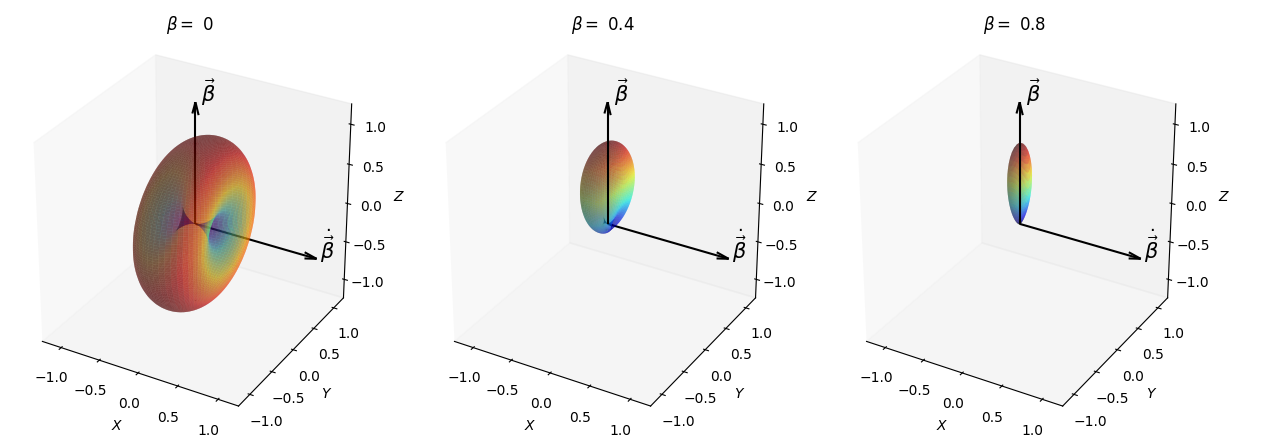
\includegraphics[scale = 0.4]{Radiation_Patterns_crop.png}\\
	\caption[Диаграми на насоченост]{Диаграми на насоченост за различни стойности на $\beta$. Диаграмите са нормирани на максималната им стойност (която се проявява при $\theta = 0$), понеже там диаграмите са разходящи при $\beta\rightarrow 1$.}
	\label{Radiation_patterns_3D}
\end{figure}

\subsection{Честотен спектър}
Сега ще пресметнем честотният спектър, измерван от далечен наблюдател. Следователно ще е по-удобно да започнем от израза (А.15) в термини на времето на \emph{засичане} $t$ и да дефинираме амплитудата $\vec{A}(t)$:
\begin{equation}
	\frac{dP(t)}{d\Omega} = \big|\vec{A}(t)\big|^2 \rightarrow \frac{dE}{d\Omega} = \int_{-\infty}^\infty \big|\vec{A}(t)\big|^2 dt
\end{equation}
Нека сега дефинираме Фурие образа на амплитудата $\vec{A}(t)$ като:
\begin{equation}
	\vec{A}(\omega) = \frac{1}{\sqrt{2\pi}}\int_\infty^\infty \vec{A}(t)e^{i\omega t}dt.
\end{equation}
Така изразът (А.19) може да се запише като:
\begin{equation}
	\frac{dE}{d\Omega} = \int_{-\infty}^\infty \big|\vec{A}(\omega)\big|^2 d\omega := \int_{0}^\infty \frac{dE}{d\omega d\Omega} d\omega,
\end{equation}
където величината $\frac{dE}{d\omega d\Omega} = \big|\vec{A}(\omega)\big|^2 + \big|\vec{A}(-\omega)\big|^2$ представлява диференциалният честотният спектър на излъчването. От тук задачата ни е да пресметнем Фурие амплитудата $\vec{A}(\omega)$, чиито израз (замествайки от (А.15)) е:
\begin{equation}
	\vec{A}(\omega) = \frac{q}{4\sqrt{2\pi^3\epsilon_0 c}}\bigintss_\infty^\infty\frac{\left\vert\vec{R}_0 \times \left[\left(\vec{R}_0 - \vec{\beta}\right)\times\dot{\vec{\beta}}\right]\right\vert^2}{(1 - \vec{\beta}\cdot\vec{R}_0)^3}e^{i\omega t}\frac{dt}{dt_0}dt_0
\end{equation}
Извършвайки смяната на променливите към $t_0$, експонентата ще се превърне в $e^{i\omega\left(t_0 + \frac{R(t_0)}{c}\right)}$. Предполагайки, че наблюдателят се намира на много голямо разстояние $|\vec{r}| >> |\vec{r}_0|$ (отново работим в отправна система, като тази във фигура \ref{Emission_Frame}) развиваме в ред $R(t_0)$:
\begin{equation}
	R(t_0) = \sqrt{r^2 + r_0^2 - 2\vec{r}\cdot\vec{r}_0}\approx r - \frac{\vec{r}}{r}\cdot\vec{r}_0 \approx r - \vec{R}_0\cdot\vec{r}_0
\end{equation}
Следствие от силната насоченост на диаграмата на излъчване е, че вектора $\vec{R}_0$ може да се приеме за константен докато максимума на диаграмата сочи към наблюдателя (т.е. докато има значително излъчване към него). С това приближение можем да запишем:
\begin{equation}
	\frac{\vec{R}_0 \times \left[\left(\vec{R}_0 - \vec{\beta}\right)\times\dot{\vec{\beta}}\right]}{(1 - \vec{\beta}\cdot\vec{R}_0)^2} = \frac{d}{dt_0}\left\{\frac{\vec{R}_0\times(\vec{R}_0\times\vec{\beta})}{1 - \vec{\beta}\cdot\vec{R}_0}\right\},
\end{equation}
което се проверява с директно пресмятане. Заместваме изразът (А.24) в (А.22) и получаваме:
\begin{eqnarray}
	\vec{A}(\omega) = \frac{q}{4\sqrt{2\pi^3\epsilon_0 c}}e^{i\frac{\omega r}{c}}\bigintsss_\infty^\infty e^{i\omega\left(t_0 - \frac{\vec{R}_0\cdot\vec{r}_0}{c}\right)}\frac{d}{dt_0}\left\{\frac{\vec{R}_0\times(\vec{R}_0\times\vec{\beta})}{1 - \vec{\beta}\cdot\vec{R}_0}\right\}dt_0
\end{eqnarray}
Интегрираме по части горният израз, като налагаме скоростта на заряда във време $t_0 = \pm\infty$ да е 0 (т.е. излъчва за \emph{краен} интервал от време). Получаваме:
\begin{equation}
	\vec{A}(\omega) = -\frac{i\omega q}{4\sqrt{2\pi^3\epsilon_0 c}}e^{i\frac{\omega r}{c}}\int_{-\infty}^\infty\vec{R}_0\times(\vec{R}_0\times\vec{\beta})e^{i\omega\left(t_0 - \frac{\vec{R}_0\cdot\vec{r}_0}{c}\right)} dt_0
\end{equation}
Известно е (и показахме в глава 2), че поляризацията на електромагнитното лъчение има 2 степени на свобода, перпендикулярни на вълновия вектор. Тогава е естествено да разложим векторното произведение в интеграла (А.26) на компоненти по $\vec{e}_{\parallel}$ и $\vec{e}_{\perp}$ (виж фигура \ref{Emission_Frame_2}).\\
\begin{minipage}{15em}
	
	\begin{tikzpicture}
		% Axes
		\draw [->] (0, 0, 0) -- (3, 0, 0) node [right] {$y$};
		\draw [->] (0, 0, 0) -- (0, 3, 0) node [left] {$z$};
		\draw [->] (0, 0,-3) -- (0, 0, 4) node [left] {$x$};
		% Vectors
		\draw [->, thick] (0, 0, 0) -- (0, 2.5, 2.5) node [right]{$\vec{R}_0$};
		\draw [->, thick] (0, 0, 0) -- (2,  0,	0) node [above]{$\vec{e}_\parallel$};
		\draw [->, thick] (0, 0, 0) -- (0, 1.5,-1.5) node [above]{$\vec{e}_\perp$};
		
		\coordinate (O) at (0, 0, 0);
		\coordinate (x) at (0, 0, 1);
		\coordinate (R0) at (0, 2.5, 2.5);
		\coordinate (arc) at (0.669872981, 0, 2.5);
		\coordinate (Оrho) at (2.8, 0, 0);
		

		\draw[canvas is xz plane at y = 0, line width = 1, domain = 220:130, -latex,blue] plot ({5 + 5 * cos(\x)}, {5 * sin(\x)});
		\draw (1.7, 0, 5) node [above]{$\vec{\beta}$};
		
		\draw [-, thick] (2.8, 0, 0) -- (0.669872981, 0, 2.5); %(5 + 5 * cos(150), 0,  5 * sin(150))
		\draw (2, 0, 2.7) node [above]{$\rho$};
		\fill  (0.669872981, 0, 2.5) circle[radius=2pt];

		\draw pic["$\psi$", draw=red, ->,angle eccentricity=1.2, angle radius = 1.5cm, transform shape] {angle = O--Оrho--arc} ;
	
		\draw pic["$\theta$", draw=red, <-,angle eccentricity=1.2, angle radius = 0.7cm, transform shape] {angle = R0--O--x} ;
	
	\end{tikzpicture}
	
	\captionsetup{font=footnotesize}
	\captionof{figure}{Локалната отправната система за разлагане на поляризацията}
	\label{Emission_Frame_2}
	
\end{minipage}
\begin{minipage}{18em}
В тази отправна система можем да разложим векторното произведение в интеграла (А.26) като:
\begin{equation}
	\begin{split}
	&\vec{R}_0\times(\vec{R_0}\times\vec{\beta}) = \\
	&\beta(-\sin\psi \vec{e}_\parallel + \cos\psi\sin\theta \vec{e}_\perp),
	\end{split}
\end{equation}
и скаларното произведение в експонентата като:
\begin{equation}
	\vec{R}_0\cdot\vec{r}_0 = \rho\cos\theta\sin\psi
\end{equation}
\end{minipage}
Ъгълът $\psi$ може да се представи като $\psi = \frac{v}{\rho}t_0$. Отчитайки, че значително излъчване в направлението $\vec{R}_0$ има само при $\theta << 1$ и $t_0 << 1$, можем да развием в ред израз (А.28) до величини от 3ти порядък:
\begin{equation}
	\cos\theta\sin\phi \approx \left(1 - \frac{\theta^2}{2}\right)\frac{v}{\rho}t_0 - \frac{v^3}{6\rho^3}t^3.
\end{equation}
Тогава можем да запишем аргумента на експонентата в (А.26) като:
\begin{equation*}
	\omega\left(t_0 - \frac{\vec{R}_0\cdot\vec{r}_0}{c}\right) = \omega\left(t_0(1-\beta) + \frac{\theta^2}{2}t_0 + \frac{c^2}{6\rho^2}t_0^3\right)\approx\frac{\omega}{2}\left[\left(\frac{1}{\gamma^2} + \theta^2\right)t_0 + \frac{c^2}{3\rho^2}t_0^3\right].
\end{equation*}
Заместваме това и (А.27) в (А.26), дефинираме новите променливи:
\begin{equation}
	x = \frac{ct_0}{\rho\sqrt{\frac{1}{\gamma^2} + \theta^2}},\quad \xi = \frac{\omega\rho}{3c}\left[\frac{1}{\gamma^2} + \theta^2\right]^{\frac{3}{2}},
\end{equation}
и получаваме за Фурие амплитудата:
\begin{equation}
	\vec{A}(\omega) = -\frac{i\omega\beta q}{4\sqrt{2\pi^3\epsilon_0 c}}\frac{\rho}{c}\sqrt{\frac{1}{\gamma^2}+\theta^2}e^{i\omega r}\bigintsss_{-\infty}^\infty\left\{\theta \vec{e}_\perp + x\sqrt{\frac{1}{\gamma^2} + \theta^2}\vec{e}_\parallel\right\}e^{i\frac{3}{2}\xi\left(x - \frac{x^3}{3}\right)}dx
\end{equation}
Нека разгледаме двата члена поотделно, започвайки с $\vec{A}_\perp$:
\begin{equation}
	\vec{A}_\perp(\omega)=-\frac{i\omega\beta q}{4\sqrt{2\pi^3\epsilon_0 c}}\frac{\rho}{c}\theta e^{i\omega r}\sqrt{\frac{1}{\gamma^2}+\theta^2}\int_{-\infty}^\infty e^{i\frac{3}{2}\xi\left(x + \frac{x}{3}\right)}dx \vec{e}_\perp
\end{equation}
За пресмятането на този интеграл ще се възползваме от интегралното представяне на функцията на Ейри $\text{Ai}(z)$, и нейната връзка с модифицираната функция на Бесел от дробен ред $\text{K}_{\frac{1}{3}}(\xi)$:
\begin{equation}
	\begin{split}
	&\int_{-\infty}^\infty e^{i\frac{3}{2}\xi\left(x + \frac{x}{3}\right)}dx = 2\pi\left(\frac{3}{2}\xi\right)^{-\frac{1}{3}}\text{Ai}\left[\left(\frac{3}{2}\xi\right)^{\frac{2}{3}}\right],\\
	&\text{Ai}(z) = \frac{1}{\pi}\sqrt{\frac{z}{3}}\text{K}_{\frac{1}{3}}(\xi),\quad z = \left(\frac{3}{2}\xi\right)^{\frac{2}{3}}.
	\end{split}
\end{equation}
Замествайки това в (А.32) можем да запишем:
\begin{equation}
	\vec{A}_\perp(\omega) = -\frac{i\omega\beta q}{2\sqrt{6\pi^3\epsilon_0 c}}\frac{\rho}{c}\theta e^{i\omega r}\sqrt{\frac{1}{\gamma^2} + \theta^2}\text{K}_{\frac{1}{3}}(\xi(\omega))\vec{e}_\perp
\end{equation}
По аналогичен начин ще запишем изразът за $\vec{A}_\parallel(\omega)$:
\begin{equation}
	\vec{A}_\parallel(\omega) = -\frac{i\omega\beta q}{4\sqrt{2\pi^3\epsilon_0 c}}\frac{\rho}{c}e^{i\omega r}\left(\frac{1}{\gamma^2} + \theta^2\right)\int_{-\infty}^\infty x e^{i\frac{3}{2}\xi\left(x + \frac{x^3}{3}\right)}dx \vec{e}_\parallel,
\end{equation}
и да се възползваме от връзката между производната на функцията не Ейри $\text{Ai}^\prime(z)$ и модифицирата функция на Бесел от дробен ред $\text{K}_{\frac{2}{3}}(\xi)$:
\begin{equation}
	\int_{-\infty}^\infty x e^{i\frac{3}{2}\xi\left(x + \frac{x^3}{3}\right)}dx = -2\sqrt{z}\text{Ai}^\prime (z) =\frac{2}{\pi}\sqrt{\frac{z}{3}}\text{K}_{\frac{2}{3}}(\xi),
\end{equation}
където $z$ има същата дефиниция като в (А.33). Заместваме (А.36) в (А.35) за да получим:
\begin{equation}
	\vec{A}_\parallel = -\frac{i\omega\rho q}{2\sqrt{6\pi^3\epsilon_0 c}}\frac{\rho}{c}e^{i\omega r}\left( \frac{1}{\gamma^2} + \theta^2 \right) \text{K}_{\frac{2}{3}}(\xi(\omega))\vec{e}_\parallel.
\end{equation}
Така връщайки се към израз (А.21) и дефиницията на диференциалният честотен спектър, можем да запишем:
\begin{equation}
	\frac{dE}{d\omega d\Omega} = \frac{q^2\beta^2}{12\pi^3\epsilon_0 c}\left(\frac{\rho\omega}{c}\right)^2\left(\frac{1}{\gamma^2}+\theta^2\right)^2\left[\text{K}^2_{\frac{2}{3}}(\xi) + \frac{\theta^2}{\frac{1}{\gamma^2} + \theta^2}\text{K}^2_{\frac{1}{3}}(\xi)\right]
\end{equation}
Интегрирайки горният израз по $\Omega$ получаваме количеството енергия, излъчена на единица честота през \emph{целият} период на излъчване. На това интегриране обаче, трябва да се обърне специално внимание. Изразът (А.38) е в термини на ъгловите координати въведени във фигура \ref{Emission_Frame_2}. Сферичната мярка тогава ще бъде $d\Omega = \cos\theta d\theta d\phi \approx \sin(\alpha + \theta) d\theta d\phi $. Където сме въвели \emph{ъгъла на усукване}, $\alpha \approx \frac{\pi}{2}$, между вектора на скоростта на заряда $\vec{\beta}$ и този на локалното магнитно поле $\vec{B}$. С това допускаме частично спираловидно движение на заряда спрямо магнитните силови линии.
\begin{equation}
	\frac{dE}{d\omega} \approx \int \frac{dE}{d\omega d\Omega} \sin(\alpha + \theta) d\theta d\phi \approx 2\pi \sin\alpha \int_{-\infty}^\infty \frac{dE}{d\omega d\Omega}d\theta:=\frac{dE}{d\omega}\bigg\vert_\parallel + \frac{dE}{d\omega}\bigg\vert_\perp.
\end{equation}
Тук отново сме използвали граничното поведение на диаграмата на излъчване при $\beta\rightarrow 1$ за да направим някой опростения:\\

\textbf{1)} Приемаме, че диаграмата е симетрична спрямо максимума си (виж фигура \ref{Radiation_patterns_3D}). Това ни позволява да интегрираме директно азимуталната част на левия интеграл в (А.39).\\

\textbf{2)} Понеже всичкото лъчение е съсредоточено в малка околност около вектора на скоростта $\vec{\beta}$, можем да приемем, че $\sin(\alpha + \theta)\approx \sin\alpha\approx\text{const}$ по време на излъчването в направление $\vec{R}_0$.  \\

\textbf{3)} Излъчването е периодично по $\theta$, но приемайки приближение (А.29) ние разглеждаме, лъчението от само една "орбита", при което математически нарушаваме периодичността. Следствие от това е появата на функции на Бесел, които асимптотично клонят към 0 при $|\theta| >> 1$. Следователно можем да разширим границите на интегриране до $\{-\infty, \infty\}$\\

Нека сега пресметнем десните величини в израз (А.39). Понеже в интеграционните променливи от изрази (А.33) и (А.36) се крие зависимост от ъгъла $\theta$, ще направим обратното на (А.30) полагане и ще въведем нова променлива $\theta^2_\gamma = \frac{1}{\gamma^2} + \theta^2$. Тогава имаме:
\begin{equation}
	\begin{split}
		&\frac{dE}{d\omega}\bigg\vert_\parallel = \frac{q^2\beta^2}{6\pi^2\epsilon_0 c}\left(\frac{\rho\omega}{c}\right)^2\sin\alpha \int_{-\infty}^\infty \theta_\gamma^4 \text{K}^2_{\frac{2}{3}}\left(\frac{\omega\rho}{3 c}\theta_\gamma^3\right)d\theta\\
		&\frac{dE}{d\omega}\bigg\vert_\perp = \frac{q^2\beta^2}{6\pi^2\epsilon_0 c}\left(\frac{\rho\omega}{c}\right)^2\sin\alpha \int_{-\infty}^\infty \theta^2\theta_\gamma^2 \text{K}^2_{\frac{1}{3}}\left(\frac{\omega\rho}{3 c}\theta_\gamma^3\right)d\theta
	\end{split}
\end{equation}
\subsubsection{Пресмятане на $\frac{dE}{d\omega}\big\vert_\parallel$}
Връщайки полагането от (А.30) в израз (А.36) и неговото комплексно спрегнато, можем да запишем $\text{K}^2_{\frac{2}{3}}\left(\frac{\omega\rho}{3 c}\theta_\gamma^3\right)$ в интегрална форма като:
\begin{equation}
\text{K}^2_{\frac{2}{3}}\left(\frac{\omega\rho}{3 c}\theta_\gamma^3\right) = 	\frac{3}{4}\frac{1}{\theta_\gamma^4}\int_{-\infty}^\infty \int_{-\infty}^\infty e^{ia\left(\theta_\gamma^2[x - y] + \frac{1}{3}[x^3 - y^3]\right)}xydxdy,
\end{equation}
където сме въвели нови променливи $x = \frac{c}{\rho}t_0$, $y = \frac{c}{\rho} t_0^\prime$, $a = \frac{\omega\rho}{2c}$. Сега извършваме още една смяна на променливите и дефинираме $2u = x + y$ $2v = x - y$. Тогава получаваме следният израз:
\begin{equation}
	\text{K}^2_{\frac{2}{3}}\left(\frac{\omega\rho}{3 c}\theta_\gamma^3\right) = 	\frac{3}{2}\frac{1}{\theta_\gamma^4}\int_{-\infty}^\infty du e^{2ia\left(\theta_\gamma^2 u + \frac{1}{3}u^3\right)}\int_{-\infty}^{\infty}\left(v^2 - u^2\right)e^{2iauv^2}dv
\end{equation}
Извършваме интегрирането по $v$, след което заместваме в (А.40) и интегрираме по $\theta$ за да получим:
\begin{equation}
	\int_{-\infty}^\infty \theta_\gamma^4 \text{K}^2_{\frac{2}{3}}\left(\frac{\omega\rho}{3 c}\theta_\gamma^3\right)d\theta = -\frac{3}{2}i\frac{\pi c}{\omega\rho}\int_{-\infty}^\infty du e^{2ia\left(\frac{u}{\gamma^2} + \frac{1}{3}u^3\right)}\left(u + \frac{c}{\omega\rho}\frac{1}{2iu^2}\right)
\end{equation}
Членът в подинтегралната функция, пропорционален на $\frac{1}{u^2}$ ще интегрираме по части за да получим:
\begin{equation}
	\int_{-\infty}^\infty \frac{1}{2iu^2}e^{2ia\left(\frac{u}{\gamma^2}+\frac{1}{3}u^3\right)}du = a\int_{-\infty}^\infty \left(\frac{1}{\gamma^2 u} + u\right)e^{2ia\left(\frac{u}{\gamma^2}+\frac{1}{3}u^3\right)}du,
\end{equation}
което заместим в (А.43) ни дава:
\begin{equation}
	\int_{-\infty}^\infty \theta_\gamma^4 \text{K}^2_{\frac{2}{3}}\left(\frac{\omega\rho}{3 c}\theta_\gamma^3\right)d\theta = -\frac{3}{2}i\frac{\pi c}{\omega\rho}\int_{-\infty}^\infty du e^{2ia\left(\frac{u}{\gamma^2} + \frac{1}{3}u^3\right)}\left(\frac{3}{2}u + \frac{1}{2\gamma^2u}\right)
\end{equation}
Ще използваме отново интегралното представяне на функциите на Ейри и Бесел за да определим първият член като:
\begin{equation}
	\int_{-\infty}^\infty u e^{2ia\left(\frac{u}{\gamma^2} + \frac{1}{3}u^3\right)}du = \frac{2i}{\sqrt{3}\gamma^2}\text{K}_{\frac{2}{3}}\left(\frac{2\omega\rho}{3c\gamma^3}\right)
\end{equation}
За да пресметнем вторият челен, нека разгледаме подобен израз (използвайки отново интегралното представяне на $\text{K}_{\frac{1}{3}}$):
\begin{equation}
	\frac{d}{d\gamma^{\prime-2}}\int_{-\infty}^{\infty}\frac{1}{u}e^{2ia\left(\frac{u}{\gamma^{\prime2}} + \frac{1}{3}u^3\right)}du = \frac{2\pi i}{\sqrt{3}}\frac{\omega\rho}{c\gamma}\text{K}_{\frac{1}{3}}\left(\frac{2\omega\rho}{3c\gamma^{\prime3}}\right).
\end{equation}
Сега е удобно да въведем т.н. \emph{критична честота} $\omega_c = \frac{3\gamma^3c}{\rho}$ и промелнивата $\eta = \frac{2\omega\rho}{3c\gamma^3}$ . В термини на тях можем да интегрираме двете страни на (A.46) по $\gamma^{\prime-2}$ за да получим:
\begin{equation}
\int_{-\infty}^{\infty}\frac{1}{u}e^{2ia\left(\frac{u}{\gamma^2} + \frac{1}{3}u^3\right)}du = -\frac{2i}{\sqrt{3}}\int_{2\frac{\omega}{\omega_c}}^{\infty} \text{K}_{\frac{1}{3}}(\eta)d\eta,
\end{equation}
като тук трябва да се отбележи следното: Границите на интегрирането по $\gamma^\prime$ са избрани $[0, \gamma]$, където $\gamma$ съответства на "оригиналната"$\,$скорост на заряда, участваща в израз (А.44). Нефизичната стойност $\gamma = 0$ е избрана с цел тъждествено да получим обратно вторият член от (А.44) (но представен в термини на известна функция). Пресмятайки го в границата $\gamma\rightarrow 0$ виждаме, че експонентата става много бързо осцилираща, което занулява тази граница на интеграла. Знакът "минус"$\,$в (А.47) идва от размяната на границите на интеграла след преминаването към променливата $\eta$.\\
Замествайки (A.47) и (A.45) в (А.44) получаваме:
\begin{equation}
		\int_{-\infty}^\infty \theta_\gamma^4 \text{K}^2_{\frac{2}{3}}\left(\frac{\omega\rho}{3 c}\theta_\gamma^3\right)d\theta = \frac{\sqrt{3}\pi c}{\omega\rho\gamma^2}\left(\frac{3}{2}\text{K}_{\frac{2}{3}}\left(2\frac{\omega}{\omega_c}\right) - \frac{1}{2}\int_{2\frac{\omega}{\omega_c}}^{\infty} \text{K}_{\frac{1}{3}}(\eta)d\eta\right).
\end{equation}
Тук е удобно да използваме рекурсивното свойство на функциите на Бесел $2\frac{d}{d\xi}\text{K}_{\frac{2}{3}}(\xi) + \text{K}_{\frac{5}{2}}(\xi) = - \text{K}_{\frac{1}{3}}(\xi)$, и да изразим (А.48) като:
\begin{equation}
		\int_{-\infty}^\infty \theta_\gamma^4 \text{K}^2_{\frac{2}{3}}\left(\frac{\omega\rho}{3 c}\theta_\gamma^3\right)d\theta = \frac{\sqrt{3}\pi c}{\gamma^2\omega\rho}\left(\text{K}_{\frac{2}{3}}\left(2\frac{\omega}{\omega_c}\right) + \int_{2\frac{\omega}{\omega_c}}^{\infty} \text{K}_{\frac{5}{3}}(\eta)d\eta\right)
\end{equation}
Заместваме това в израз (А.40) и получаваме крайният резултат:
\begin{equation}
	\boxed{\frac{dE}{d\omega}\bigg\vert_\parallel = \frac{\sqrt{3}q^2\beta^2}{8\pi\epsilon_0 c}\gamma\sin\alpha\left[\text{F}\left(2\frac{\omega}{\omega_c}\right) + \text{G}\left(2\frac{\omega}{\omega_c}\right)\right]}\,,
\end{equation}
където сме въвели функциите:
\begin{equation}
	\begin{split}
	&\text{F}(x) = x\int_x^{\infty}\text{K}_{\frac{5}{3}}(\eta)d\eta\\
	&\text{G}(x) = x\text{K}_{\frac{2}{3}}(x)
	\end{split}
\end{equation}
\subsubsection{Пресмятане на $\frac{dE}{d\omega}\big\vert_\perp$}
Подхождаме поп същият начин към изразяването на  $\text{K}^2_{\frac{1}{3}}\left(\frac{\omega\rho}{3 c}\theta_\gamma^3\right)$ в интегрална форма:
\begin{equation}
	\text{K}^2_{\frac{1}{3}}\left(\frac{\omega\rho}{3 c}\theta_\gamma^3\right) = 	\frac{3}{4}\frac{1}{\theta_\gamma^2}\int_{-\infty}^\infty \int_{-\infty}^\infty e^{ia\left(\theta_\gamma^2[x - y] + \frac{1}{3}[x^3 - y^3]\right)}dxdy
\end{equation}
Отново въвеждаме променливите $2u = x + y$ $2v = x - y$, заместваме в (А.52) и получаваме:
\begin{equation}
	\text{K}^2_{\frac{1}{3}}\left(\frac{\omega\rho}{3 c}\theta_\gamma^3\right) = 	\frac{3}{2}\frac{1}{\theta_\gamma^2}\int_{-\infty}^\infty du e^{2ia\left(\theta_\gamma^2 u + \frac{1}{3}u^3\right)}\int_{-\infty}^{\infty}e^{2iauv^2}dv.
\end{equation}
Този израз заместваме в (А.40) и извършваме интегриране по $v$, и после по $\theta$ за да получим:
\begin{equation}
	\int_{-\infty}^\infty \theta^2\theta_\gamma^2 \text{K}^2_{\frac{1}{3}}\left(\frac{\omega\rho}{3 c}\theta_\gamma^3\right)d\theta = -\frac{3\pi}{4}\left(\frac{c}{\omega\rho}\right)^2\int_{-\infty}^{\infty}\frac{1}{u^2} e^{2ia\left(\frac{u}{\gamma^2}+\frac{1}{3}u^3\right)}du
\end{equation}
Този израз вече пресметнахме в (А.44), Тогава можем директно да заместим изрази (А.46) и (А.48) за да получим:
\begin{equation}
	\int_{-\infty}^\infty \theta^2\theta_\gamma^2 \text{K}^2_{\frac{1}{3}}\left(\frac{\omega\rho}{3 c}\theta_\gamma^3\right)d\theta = \frac{\sqrt{3}\pi}{2}\frac{c}{\omega\rho \gamma^2}\left[\text{K}_{\frac{2}{3}}\left(2\frac{\omega}{\omega_c}\right) - \int_{2\frac{\omega}{\omega_c}}^\infty \text{K}_{\frac{1}{3}}(\eta)d\eta\right].
\end{equation}
Тук отново ще заместим $2\frac{d}{d\xi}\text{K}_{\frac{2}{3}}(\xi) + \text{K}_{\frac{5}{2}}(\xi) = - \text{K}_{\frac{1}{3}}(\xi)$ за да получим крайният израз:
\begin{equation}
	\boxed{\frac{dE}{d\omega}\bigg\vert_\perp = \frac{\sqrt{3}q^2\beta^2}{8\pi\epsilon_0 c}\gamma\sin\alpha\left[\text{F}\left(2\frac{\omega}{\omega_c}\right) - \text{G}\left(2\frac{\omega}{\omega_c}\right)\right]}
\end{equation}
\subsection{Функции на излъчване в Стоксов базис}

\end{appendices}
